\section{Overview}
\label{sec:overview}

\subsection{A brief introduction to Information Retrieval and the merits of Video-Text Retrieval}
%  paragraph 1
In recent years, we are witnessing impressive growth in both computer hardware and software, which have contributed to the outcomes’ improvement of many expensive tasks, including search.
Information Retrieval (IR), or search in common, is a long-history task claimed to appear in the third century BC in an early type relevant to library administration \cite{eliot2009companion}.
What people know of this terminology today is usually related to electronic devices and the Internet. For example, we may seek a friend’s name in a phonebook or look for a song from its lyrics, a movie from its content by using some search engines.
When we do not know something, instead of going to the library or any kind of information center like we did in the past, most of us constantly “google” it at first.
All of those examples, in fact, are associated with something called Information Retrieval System (IRS) - the implementation of any specific IR theory into the computer operation.
An IR system feeds a query in a particular type as input and gives back the most relevant results to the user through automatic matching methods between the input and data sources (see figure \ref{fig:IR_structure}).
\begin{figure}[!t]
    \centering
    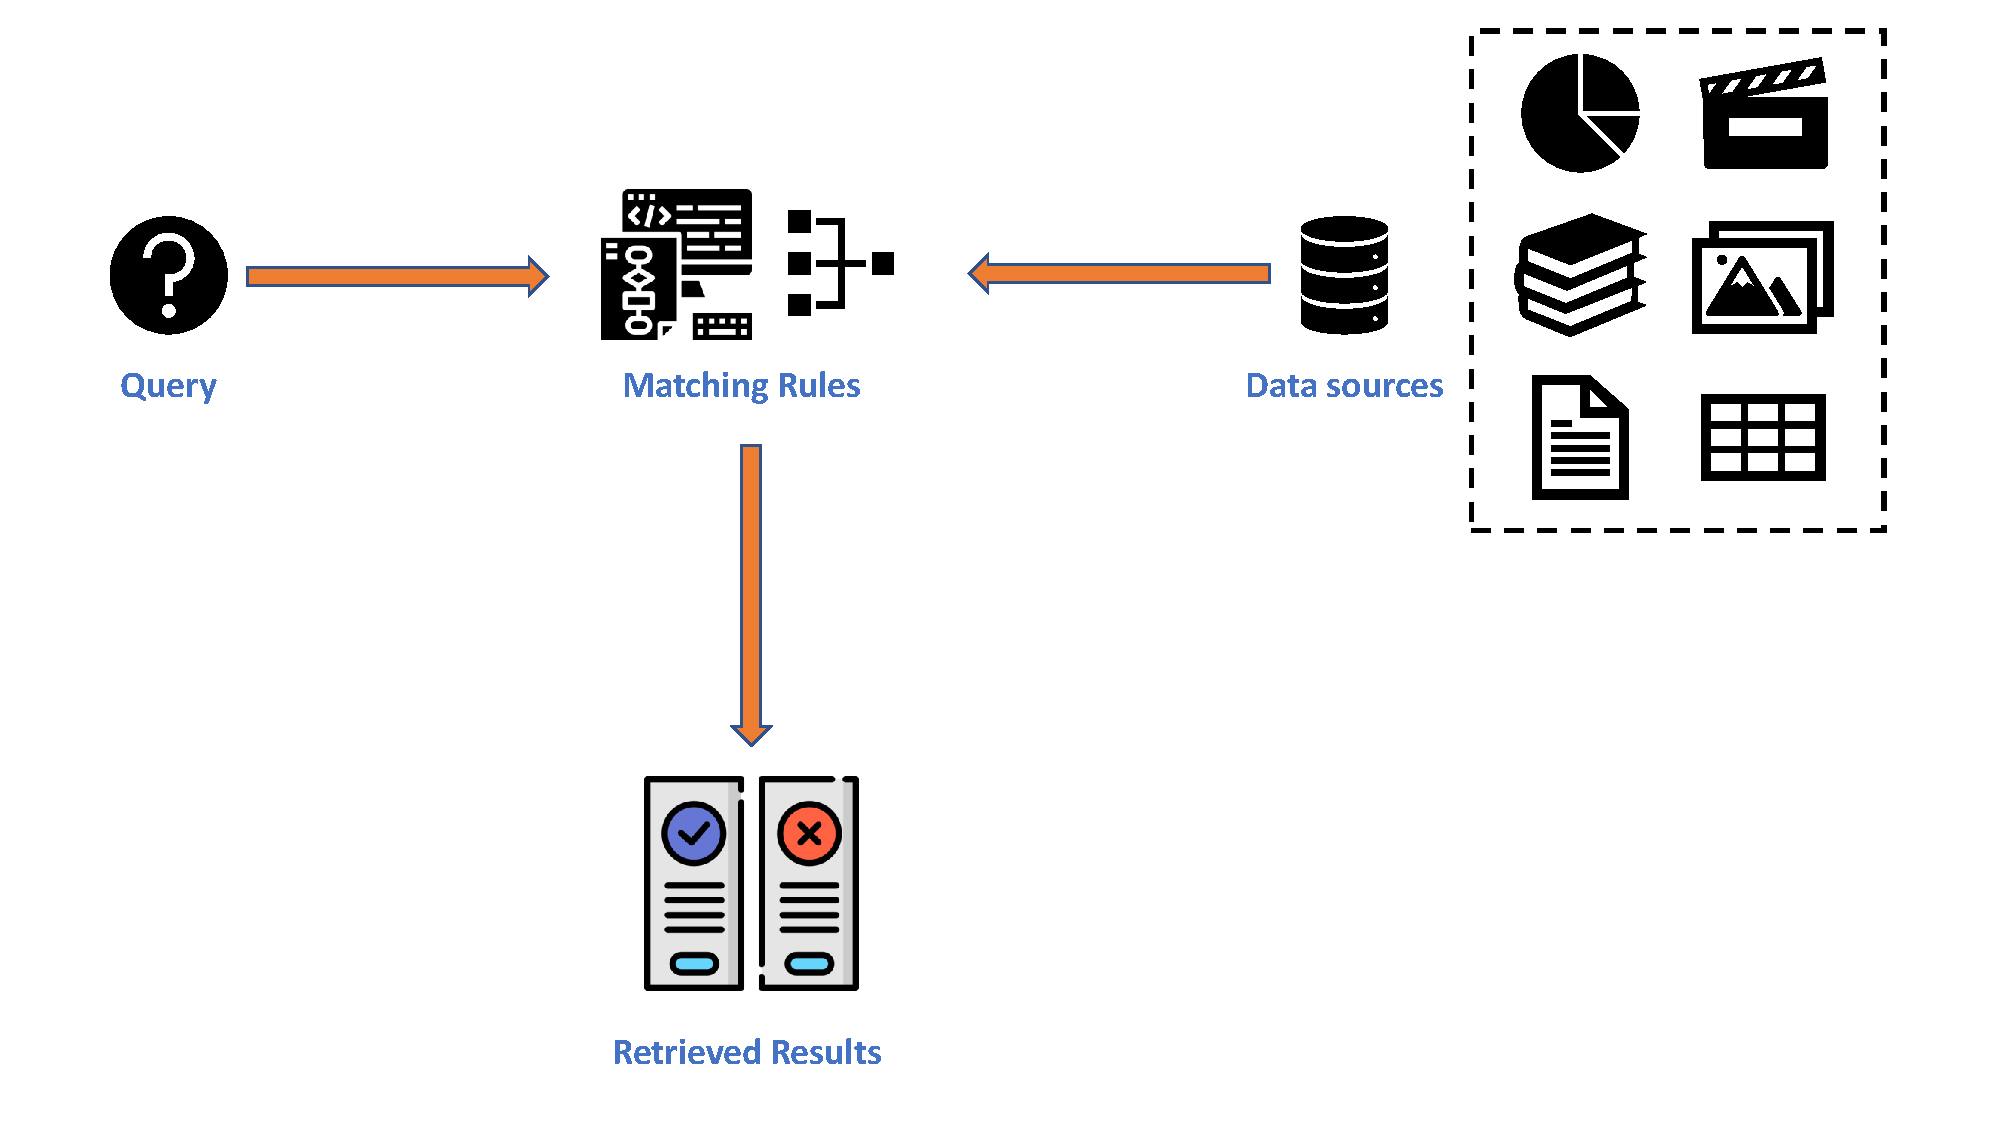
\includegraphics[width=\linewidth]{resources/images/overview/IR_structure.pdf}
    \caption{A simple overview of the Information Retrieval System}
    \label{fig:IR_structure}
\end{figure}
The need for such things occurred due to the increasingly rapid rise in data size and various kinds of information in different areas (like multimedia, website, scientific publication, etc.), making traditional searching techniques no longer cope.
In any IRS, there are always two aspects to deal with: system operation and matching algorithms. Since the first application in the 1940s, it has been developed continuously until now, with many essential milestones \cite{sanderson2012history} tackling both aspects.

%  paragraph 2
As the computing environment changes from time to time, many applications of IR have been suggested, like search on social networks, desktop element search, or one research hotspot recently named cross-modal retrieval.
This task aims to pick out relevant data across different modalities, such as image-text, video-text, audio-text.
Maragos et al. \cite{maragos2008multimodal} stated two future challenges with multimodal applications, including (i) Natural access and high-level interaction with multimedia databases and (ii) Detecting, recognizing and interpreting objects, events and human behavior in multimedia videos by processing combined audio-video-text data.
This statement also reflects two aspects that people always deal with the IRS, as mentioned above.
In research, people may care more about the method aspect than the other.
Traditional methods with manually designed representations, features and matching functions lack the ability to tackle complex IR tasks like multimodal interaction when those tasks require a deeper understanding of document contents and the user information needed \cite{culpepper2018research}.
However, thanks to an ever-stronger influence of Deep Learning \cite{goodfellow2016deep,lecun2015deep} in the 2010s decade, many problems raised in this field have resulted in better performance, letting people expect a new generation of robust and intelligent cross-modal Information Retrieval Systems.

%  paragraph 3
Also, humans have recently witnessed a rapid explosion in the appearance of videos in many aspects of their daily lives.
We all know the potential of videos in entertainment, communication, data analysis, etc.
The rise of video-based online services like YouTube, Netflix, along with the traditional TV program, has inspired Computer Vision (CV) experts to pay more attention to this resource. Additionally, natural language (NL) is one of the most effective means to describe those video contents.
From this point of view, the task of searching videos via text queries, or video-text retrieval, in short, becomes a desirable function in intelligent systems.
This problem takes (a) natural language text description(s) as input and outputs a sorted list of videos in terms of semantic relevance.
A lot of neuron network-based methods, focusing on transforming text input and video’s particular contents into the same subspace and measuring their similarity, have worked efficiently.
However, each video retrieval task has its own specificities among the diversity of the visual world, besides some in-tackling challenges like the semantic gap between two modalities, lack of annotated video-caption, or complicated consideration of temporal information, making no universal utilization approach fit for all such retrieval problems.
Therefore, caption-to-video retrieval is still attracting researchers to resolve in different areas.

\subsection{A brief introduction to Intelligent Transportation/Traffic System and the merits of Vehicle-oriented Computer Vision Tasks}
%  paragraph 1
Transportation is a non-separable part of any country, playing an essential role in different aspects of our daily life.
Residents, governments, and businesses almost depend on it to access resources.
Therefore, the advent of Intelligent Transportation/Traffic System (ITS), a significant factor contributing to the concept of smart city and to the development of modern civilization, is inevitable.
The implementation of ITS is widely accepted and used in many countries today when the governments recognize (i) the rapid growth of the human population, (ii) high-speed urbanization, and (iii) increasing vehicle ownership.
Though there are multiple modes of transportation, the roadway is the most common route.
So this kind of system aims to address a wide range of road traffic issues via advanced technologies, solving at three main levels: society, the road administrator, and drivers.
By providing different modules centering around the people-vehicle-road relation, and other traffic objects, it helps improve the safety, efficiency,  and environmental friendliness of the transportation.

%  paragraph 2
In an ITS that inherits Deep Learning works, Fan et al. \cite{fan2020deep} have shown that there are four major services in the architecture, as illustrated in figure \ref{fig:ITS_structure}.
\begin{figure}[!t]
    \centering
    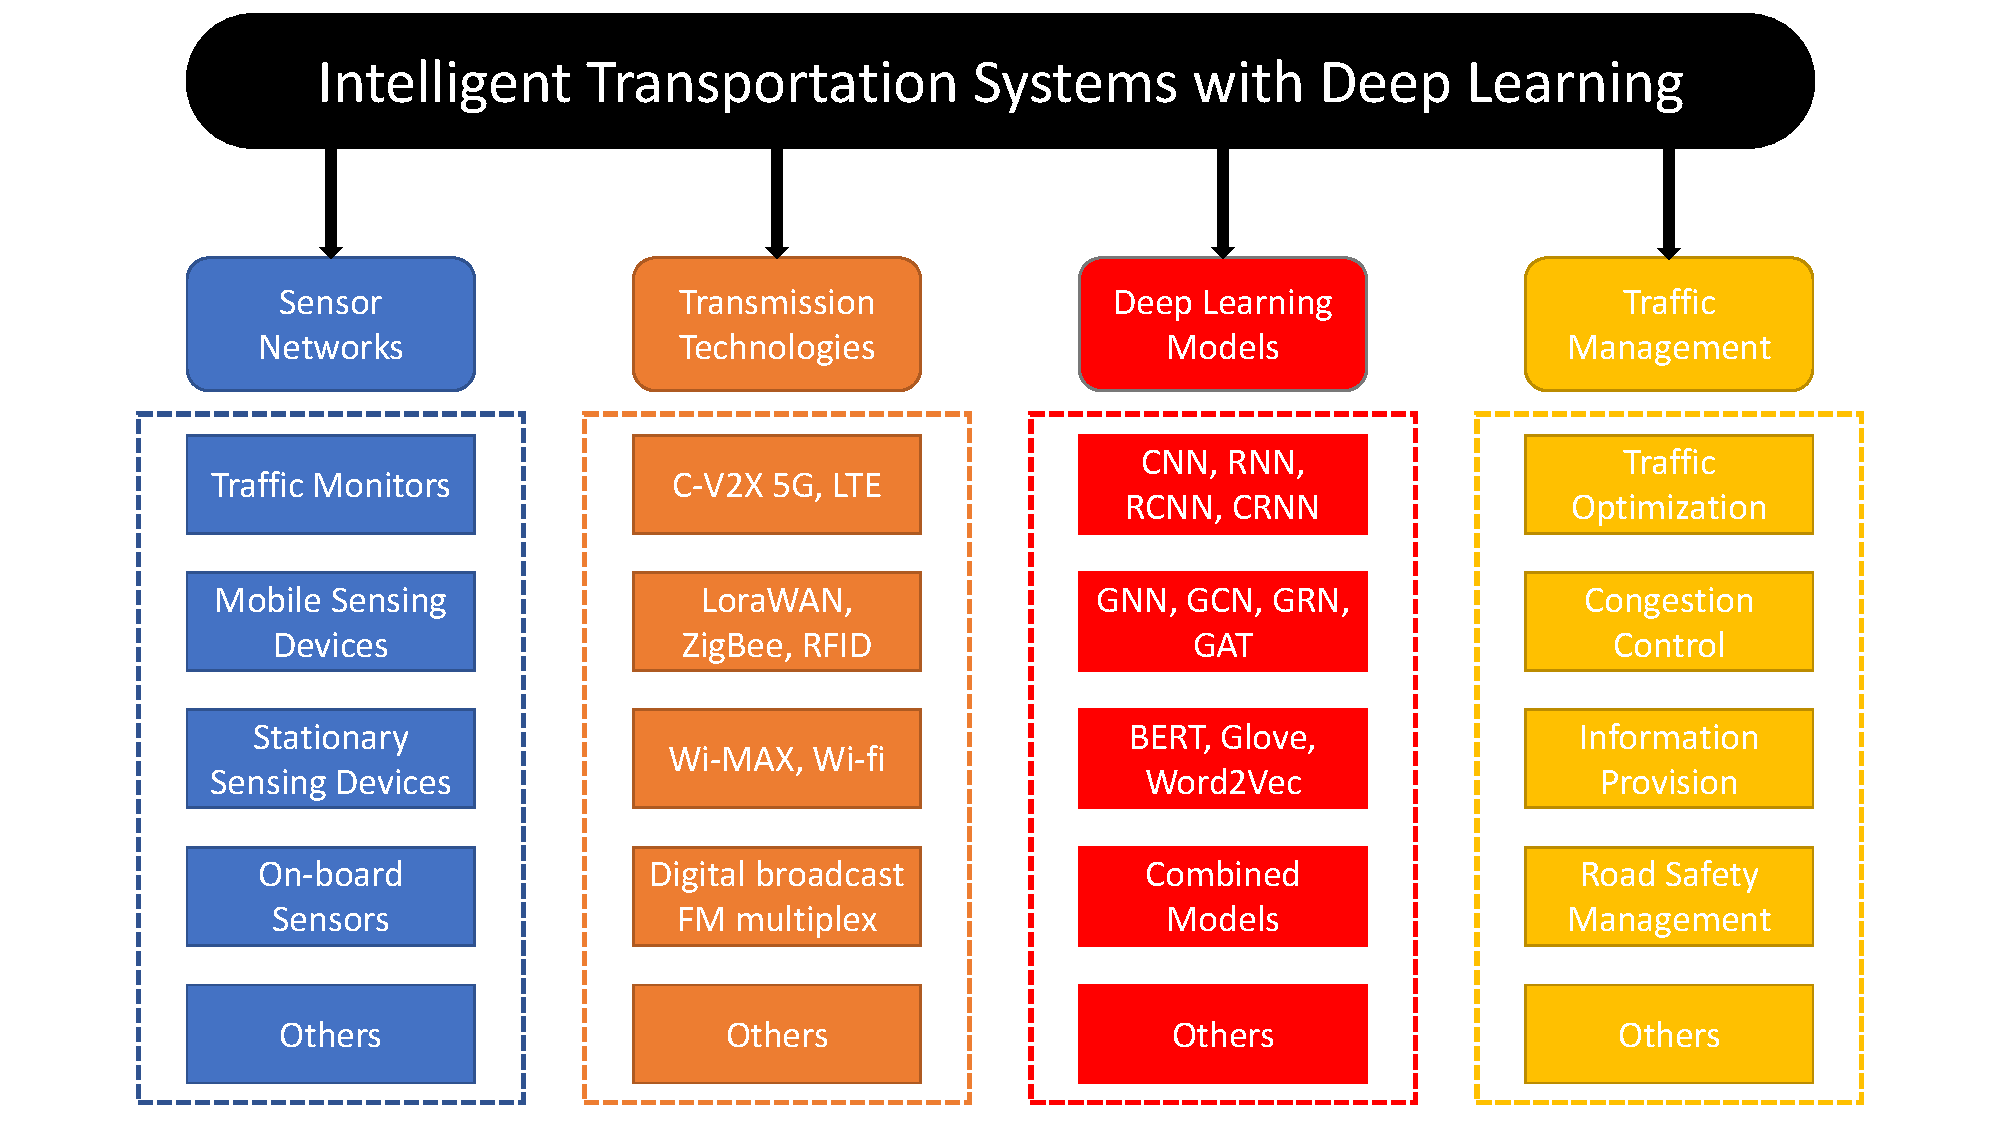
\includegraphics[width=\linewidth]{resources/images/overview/ITS_structure.pdf}
    \caption{Major components of a Deep Learning-based Intelligent Transportation/Traffic System.}
    \label{fig:ITS_structure}
\end{figure}
The Sensor Networks service is in charge of collecting real-time data then sends it through the Transmission Technologies service.
By exploiting the data, the Deep Learning Models service is responsible for building models that can perform well in particular tasks before integrating them into practical modules of the Traffic Management service.
When it comes to Computer Vision applications in such systems, many problems are mainly related to vehicles.
This is because transportation is vehicle-centered, unlike other areas, which are often people-focused.
Thanks to the widespread installment of 24/7 surveillance cameras on roads and highways, people can obtain massive traffic data.
Although the potential for video analytics from that data is enormous to be leveraged, it has not been exploited optimally.
Some tasks have received high-accurate state-of-the-art results, such as Vehicle Counting \cite{lu2021robust, dai2019video, asha2018vehicle} or Vehicle Reidentification \cite{luo2021empirical, Khorramshahi_2019_ICCV, zhu2019vehicle}, but some are still far from saturated outcomes.
Two major hurdles include the insufficiency of labels and the lack of high-performance models capable of converting data into valuable insights.
Regarding the model, since the vehicle is a particular domain and non-human, many pre-trained models cannot be applied directly to this object.
Therefore, CV researchers in this field still face so many significant challenges.
And, there should be something that can attract attention to address such issues.

%  paragraph 3
For those reasons, in parallel with the works of individuals, there are also organizations holding vehicle-oriented contests in order to find solutions from talented candidates.
Not stopping there, through these contests, people hope for deployments of submitted models into a realistic environment. 
One of the hottest contests is the AI City Challenge \cite{Naphade17AIC17, Naphade18AIC18, Naphade19AIC19, Naphade20AIC20, Naphade21AIC21}, opening continuously since 2017.
This contest primarily focuses on accurate, robust, and efficient approaches, so the organizers provide relatively sufficient labeled datasets \cite{Feng21CityFlowNL, Tang19CityFlow, Yao20VehicleX} as well as the evaluation system.
Their problems range from the mentioned tasks above to others like Velocity Estimation, Anomaly Detection, Vehicle Tracking, etc., whose insights may be inspired by various techniques.
In the latest edition, the 5th AI City Challenge \cite{Naphade21AIC21} has proposed a novel advanced track named Natural Language-Based Vehicle Retrieval (NL-based VR), which needs an effective combination of subtasks including motion detection, appearance recognition and content-based video retrieval.
There are still other tasks from other competitions, but finally, they all have the same goal: to solve real-world traffic issues and implement them into the Intelligent Transportation/Traffic System.